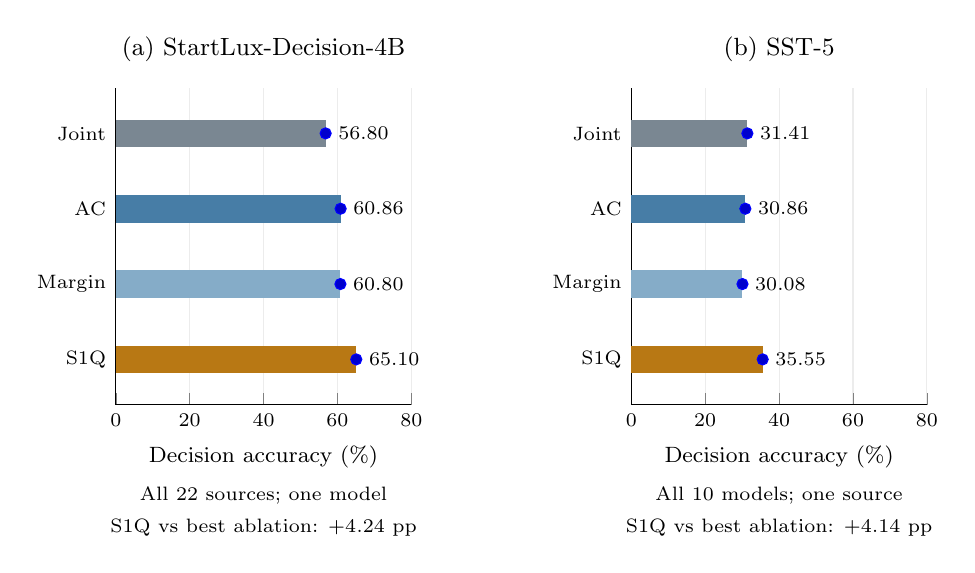
\begin{tikzpicture}
\begin{axis}[width=.44\textwidth,height=5.6cm,xmin=0,xmax=80,
ymin=-.6,ymax=3.6,xtick={0,20,40,60,80},ytick={0,1,2,3},yticklabels={S1Q,Margin,AC,Joint},
xlabel={Decision accuracy (\%)},bar width=10pt,axis lines*=left,xmajorgrids,grid style={gray!15},
tick label style={font=\scriptsize},label style={font=\footnotesize},clip=false,
title={(a) StartLux-Decision-4B},title style={font=\small}]
\definecolor{casecolor00}{HTML}{7A8792}
\addplot+[xbar,bar shift=0pt,fill=casecolor00,draw=none,forget plot] coordinates {(56.8034334028,3)};
\node[anchor=west,font=\scriptsize] at (axis cs:57.6034334028,3) {56.80};
\definecolor{casecolor01}{HTML}{477DA6}
\addplot+[xbar,bar shift=0pt,fill=casecolor01,draw=none,forget plot] coordinates {(60.8582251684,2)};
\node[anchor=west,font=\scriptsize] at (axis cs:61.6582251684,2) {60.86};
\definecolor{casecolor02}{HTML}{85ACC8}
\addplot+[xbar,bar shift=0pt,fill=casecolor02,draw=none,forget plot] coordinates {(60.8026970020,1)};
\node[anchor=west,font=\scriptsize] at (axis cs:61.6026970020,1) {60.80};
\definecolor{casecolor03}{HTML}{B87814}
\addplot+[xbar,bar shift=0pt,fill=casecolor03,draw=none,forget plot] coordinates {(65.0967565305,0)};
\node[anchor=west,font=\scriptsize] at (axis cs:65.8967565305,0) {65.10};
\node[anchor=north,font=\scriptsize] at (rel axis cs:.5,-.23) {All 22 sources; one model};
\node[anchor=north,font=\scriptsize] at (rel axis cs:.5,-.33) {S1Q vs best ablation: $+4.24$ pp};
\end{axis}
\begin{axis}[at={(.54\textwidth,0)},anchor=south west,width=.44\textwidth,height=5.6cm,xmin=0,xmax=80,
ymin=-.6,ymax=3.6,xtick={0,20,40,60,80},ytick={0,1,2,3},yticklabels={S1Q,Margin,AC,Joint},
xlabel={Decision accuracy (\%)},bar width=10pt,axis lines*=left,xmajorgrids,grid style={gray!15},
tick label style={font=\scriptsize},label style={font=\footnotesize},clip=false,
title={(b) SST-5},title style={font=\small}]
\definecolor{casecolor10}{HTML}{7A8792}
\addplot+[xbar,bar shift=0pt,fill=casecolor10,draw=none,forget plot] coordinates {(31.4062500000,3)};
\node[anchor=west,font=\scriptsize] at (axis cs:32.2062500000,3) {31.41};
\definecolor{casecolor11}{HTML}{477DA6}
\addplot+[xbar,bar shift=0pt,fill=casecolor11,draw=none,forget plot] coordinates {(30.8593750000,2)};
\node[anchor=west,font=\scriptsize] at (axis cs:31.6593750000,2) {30.86};
\definecolor{casecolor12}{HTML}{85ACC8}
\addplot+[xbar,bar shift=0pt,fill=casecolor12,draw=none,forget plot] coordinates {(30.0781250000,1)};
\node[anchor=west,font=\scriptsize] at (axis cs:30.8781250000,1) {30.08};
\definecolor{casecolor13}{HTML}{B87814}
\addplot+[xbar,bar shift=0pt,fill=casecolor13,draw=none,forget plot] coordinates {(35.5468750000,0)};
\node[anchor=west,font=\scriptsize] at (axis cs:36.3468750000,0) {35.55};
\node[anchor=north,font=\scriptsize] at (rel axis cs:.5,-.23) {All 10 models; one source};
\node[anchor=north,font=\scriptsize] at (rel axis cs:.5,-.33) {S1Q vs best ablation: $+4.14$ pp};
\end{axis}
\end{tikzpicture}
